\chapter{Results}
\label{ch:results}
This chapter presents the findings from my research into the use of LLMs for classifying and transferring between German language proficiency levels. The results are organized according to the two main tasks: CEFR classification and proficiency level transfer. I first present the outcomes of the classification tasks using both prompt engineering and fine-tuning approaches. This is then followed by the results of my text transfer experiments. For each set of results, I provide quantitative metrics, visualizations and a brief description of key findings.

\section{Classification Dataset Analysis}
\label{s:classification_dataset_analysis}
\subsection*{Dataset Composition}
\label{ss:dataset_composition}
The classification dataset consists of 1,445 text samples across all six CEFR levels (A1,A2,B1,B2,C1,C2). The distribution of the samples across the different levels is shown in Table \ref{tab:data_distribution}. Notably, the distribution is not uniform across all levels - A2, B1 and B2 have a higher representation (306, 331, 376 samples respectively) compared to A1, C1 and C2 (179, 179, 196 samples respectively). This imbalance results primarily from the scarce availability of data in the source datasets and current inability to generate high-quality synthetic data for the higher CEFR levels.
\subsection*{Word Count Distribution}
\label{ss:word_count_distribution}An analysis of the word count across different CEFR levels shows interesting patterns, seen in Figure \ref{fig:word-count-distribution} and Table \ref{tab:word_count_statistics}. The A1 level shows a rather high average word count (594.98 words) in comparison to A2. This is due to the synthetic data generation process, which aimed to create texts around the 600-word mark. \\
There also emerges a clear trend of increasing average word count for the higher CEFR levels, with C2 having the highest average word count (2,832,37 words). This aligns with exceptions, as higher CEFR levels are typically much more complex and thus tend to have longer texts. The word count variance is also significantly higher for the higher CEFR levels, with C2 having a variance of 1,152.74 words.
\begin{figure}
    \centering
    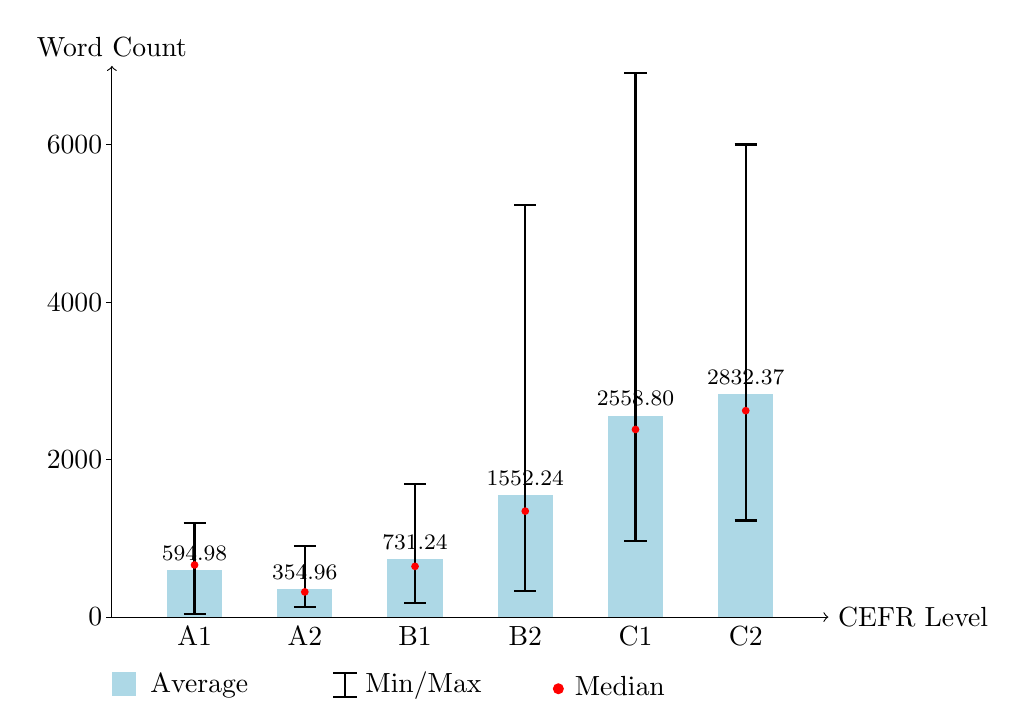
\begin{tikzpicture}[scale=0.7]
        % Define colors
        \definecolor{barcolor}{RGB}{173,216,230}
        
        % Draw axes
        \draw[->] (0,0) -- (13,0) node[right] {CEFR Level};
        \draw[->] (0,0) -- (0,10) node[above] {Word Count};
        
        % Y-axis labels
        \foreach \y in {0,2000,4000,6000}
            \draw (0,\y/700) node[left] {\y} -- (-0.1,\y/700);
        
        % Data
        \foreach [count=\i] \x/\y/\min/\max/\med in {
            A1/594.98/44/1198/662,
            A2/354.96/126/901/319.5,
            B1/731.24/183/1692/644,
            B2/1552.24/330/5230/1345.5,
            C1/2558.80/967/6910/2382.5,
            C2/2832.37/1227/6001/2621.5
        } {
            % Draw bar
            \fill[barcolor] (2*\i-1,0) rectangle (2*\i,\y/700);
            % Draw error bars
            \draw[thick] (2*\i-0.5,\min/700) -- (2*\i-0.5,\max/700);
            \draw[thick] (2*\i-0.7,\min/700) -- (2*\i-0.3,\min/700);
            \draw[thick] (2*\i-0.7,\max/700) -- (2*\i-0.3,\max/700);
            % Draw median marker
            \fill[red] (2*\i-0.5,\med/700) circle (2pt);
            % Labels
            \node[below] at (2*\i-0.5,0) {\x};
            \node[above] at (2*\i-0.5,\y/700) {\footnotesize\y};
        }
        
        % Spaced and Fixed Legend
        \node[below right, inner sep=0, outer sep=0] at (0,-1) {
            \tikz\fill[barcolor] (0,0) rectangle (0.3,0.3);
        };
        \node[right, inner sep=0, outer sep=0] at (0.7,-1.25) {Average};
        
        \node[below right, inner sep=0, outer sep=0] at (4,-1) {
            \tikz{
                \draw[thick] (0,0) -- (0.3,0);    % Bottom horizontal line
                \draw[thick] (0,0.3) -- (0.3,0.3); % Top horizontal line
                \draw[thick] (0.15,0) -- (0.15,0.3); % Vertical line
            }
        };
        \node[right, inner sep=0, outer sep=0] at (4.6,-1.25) {Min/Max};
        
        \node[below right, inner sep=0, outer sep=0] at (8,-1.2) {
            \tikz\fill[red] (0.15,0.15) circle (2pt);
        };
        \node[right, inner sep=0, outer sep=0] at (8.4,-1.25) {Median};
        
    \end{tikzpicture}
    \caption{Word Count Distribution Across CEFR Levels}
    \label{fig:word-count-distribution}
\end{figure}

\begin{table}[ht]
    \centering
    \begin{tabular}{
        >{\raggedright\arraybackslash}p{2cm}
        >{\raggedright\arraybackslash}p{2cm}
        >{\raggedright\arraybackslash}p{2cm}
        >{\raggedright\arraybackslash}p{2cm}
        >{\raggedright\arraybackslash}p{2cm}
        >{\raggedright\arraybackslash}p{2.5cm}
        }
        \toprule
        \textbf{CEFR Level} & \textbf{Average} & \textbf{Minimum} & \textbf{Maximum} & \textbf{Median} & \textbf{Standard Deviation\textsuperscript{*}} \\
        \midrule
        A1 & 594.98 & 44 & 1,198 & 662.00 & 299.93 \\ \midrule
        A2 & 354.96 & 126 & 901 & 319.50 & 140.51 \\ \midrule
        B1 & 731.24 & 183 & 1,692 & 644.00 & 315.86 \\ \midrule
        B2 & 1,552.24 & 330 & 5,230 & 1,345.50 & 754.68 \\ \midrule
        C1 & 2,558.80 & 967 & 6,910 & 2,382.50 & 1,152.74 \\ \midrule
        C2 & 2,832.37 & 1,227 & 6,001 & 2,621.50 & 956.47 \\
        \bottomrule
    \end{tabular}
    \raggedright
    \small
    \textsuperscript{*}Standard Deviation is calculated using the formula: $\sigma = \sqrt{\frac{1}{n}\sum_{i=1}^n (x_i - \mu)^2}$, where $\sigma$ is the standard deviation, $n$ the number of samples, $x_i$ the individual word counts, and $\mu$ the mean word count.
    \caption{Word Count Statistics Across CEFR Levels}
    \label{tab:word_count_statistics}
\end{table}

Having analyzed the composition and characteristics of the dataset, I can now proceed to examine how the models perform in classifying and transferring between CEFR levels. The imbalanced distribution of samples across levels, especially the overrepresentation of B1 and B2 levels may influence the model's performance. In the following sections, I'll present the results of the classification and transfer tasks while keeping these dataset characteristics in mind.

\section{Classification Task Results}
\label{s:classification_results}

\subsection{Prompt Engineering Approaches}
\label{ss:prompt_engineering_results}

\subsubsection*{Performance Comparison of Different Prompts}
\label{sss:prompt_performance_comparison}
Figure \ref{fig:prompt-accuracy-comparison} shows the performance comparison across three prompt generations for classification of sample texts. A clear progression in both accuracy and group accuracy is evident as I refined the prompt. The basic English prompt, my initial approach, showed the lowest performance with 23.3\% accuracy and 64.6\% group accuracy. Switching to German prompts showed significant improvement. The German Zero-Shot approach increased accuracy to 33.3\% and group accuracy to 75.3\%, highlighting the importance of language alignment between prompt and target texts.
The German Few-Shot prompt demonstrated the most substantial performance boost, achieving 59.3\% accuracy and 94.0\% group accuracy. This approach nearly doubled the accuracy of the German Zero-Shot method and significantly increased group accuracy.
These results confirm the effectiveness of few-shot learning in this context. The high group accuracy of the German Few-Shot prompt is also noteworthy, indicating strong performance in identifying correct or adjacent CEFR levels.

\begin{figure}
    \centering
    \begin{tikzpicture}[scale=0.6]
        % Define colors
        \definecolor{accuracycolor}{RGB}{31,119,180}
        \definecolor{groupaccuracycolor}{RGB}{255,127,14}
        % Draw axes
        \draw[->] (0,0) -- (12,0) node[right] {Prompt Type};
        \draw[->] (0,0) -- (0,11) node[above] {Accuracy (\%)};
        % Y-axis labels
        \foreach \y in {0,20,40,60,80,100}
            \draw (0,\y/10) node[left] {\y} -- (-0.1,\y/10);
        % Data
        \foreach [count=\i] \prompttype/\accuracy/\groupaccuracy in {
            {Basic English}/23.3/64.6,
            {German Zero-Shot}/33.3/75.3,
            {German Few-Shot}/59.3/94.0
        } {
            % Draw bars
            \fill[accuracycolor] (3.8*\i-2.8,0) rectangle (3.8*\i-1.55,\accuracy/10);
            \fill[groupaccuracycolor] (3.8*\i-1.5,0) rectangle (3.8*\i-0.25,\groupaccuracy/10);
            % Labels
            \node[below, text width=3cm, align=center, rotate=30, anchor=north east] at (3.8*\i+0.5,0) {\footnotesize\prompttype};
            \node[above right, xshift=2pt] at (3.8*\i-3.3,\accuracy/10) {\footnotesize\accuracy\%};
            \node[above right, xshift=2pt] at (3.8*\i-1.8,\groupaccuracy/10) {\footnotesize\groupaccuracy\%};
        }
        % Legend
        % \node[anchor=north west, inner sep=0] at (12.5,11) {
        % \begin{tikzpicture}[baseline]
        %     \fill[accuracycolor] (0,0.7) rectangle (0.3,1);
        %     \node[anchor=west] at (0.5,0.85) {Accuracy};
        %     \fill[groupaccuracycolor] (0,0) rectangle (0.3,0.3);
        %     \node[anchor=west] at (0.5,0.15) {Group Accuracy};
        % \end{tikzpicture}
        \node[anchor=north west, inner sep=0, outer sep=0] at (3,11) {
            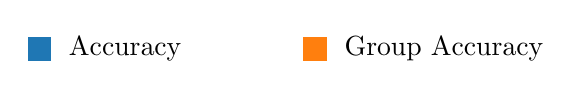
\begin{tikzpicture}
            \fill[accuracycolor] (0,0) rectangle (0.3,0.3);
            \node[right] at (0.4,0.15) {Accuracy};
            \fill[groupaccuracycolor] (3.5,0) rectangle (3.8,0.3);
            \node[right] at (3.9,0.15) {Group Accuracy};
        \end{tikzpicture}
        };
    \end{tikzpicture}
    \caption{Accuracy Comparison Across Different Prompt Generations}
    \label{fig:prompt-accuracy-comparison}
\end{figure}

\subsubsection*{Detailed Evaluation of Best Performing Prompt}
\label{sss:best_prompt_evaluation}

The German Few-Shot prompt, which demonstrated the best performance in the previous benchmarks, was further evaluated to provide a detailed analysis of its classification capabilities.
Table \ref{tab:few_shot_confusion_matrix} shows the confusion matrix for the German Few-Shot prompt, with a sample size of 25 texts per CEFR level. Notably, the majority of predictions align along the diagonal of the matrix, indicating a strong tendency for correct classifications. This alignment is a good indicator for the model's performance, as it suggests that the model is consistently identifying the correct CEFR level across different classes.

\begin{table}[ht]
    \centering
    \begin{tabular}{c|ccc}
        & \multicolumn{3}{c}{\textbf{Metrics}} \\
        Class & Precision & Recall & F1 Score \\
        \hline
        A1 & 0.8333 & 0.6000 & 0.6977 \\
        A2 & 0.6000 & \cellcolor[rgb]{1,0.9,0.9}0.3600 & \cellcolor[rgb]{1,0.9,0.9}0.4500 \\
        B1 & \cellcolor[rgb]{1,0.9,0.9}0.4706 & 0.6400 & 0.5424 \\
        B2 & 0.5676 & 0.8400 & 0.6774 \\
        C1 & 0.5455 & \cellcolor[rgb]{1,0.9,0.9}0.2400 & \cellcolor[rgb]{1,0.9,0.9}0.3333 \\
        C2 & 0.6286 & 0.8800 & 0.7333 \\
    \end{tabular}
    \caption{Performance Metrics for CEFR Classification using German Few-Shot Prompt}
    \label{tab:cefr_performance_metrics}
\end{table}

Further insights can be gained from the precision, recall and F1 scores for each CEFR level, as presented in Table \ref{tab:cefr_performance_metrics}. The model demonstrates varying performance across different levels:
\begin{enumerate}
    \item A1 level shows the highest precision (83.33\%) but moderate recall (60\%), suggesting the model has a more conservative approach to classifying texts at this level.
    \item B2 and C2 levels show balanced performance with high recall (84\% and 88\% respectively) and moderate precision, resulting in the highest F1 scores among all levels (67.74 and 73.33).
    \item A2 and C1 levels present the most challenging classifications, with lower recall scores (36\% and 24\% respectively), indicating difficulties in identifying these intermediate levels between the extremes and central levels.
    \item B1 level shows a balance between precision and recall, but both metrics are relatively low, suggesting consistent but moderate performance for this level.
\end{enumerate}

These results highlight the model's strengths in identifying extreme levels (A1 and C2) and the B2 level, while also revealing challenges in distinguishing between adjacent intermediate levels. The lower performance on A2 and C1 levels may be due to their transitional nature, making them harder to distinguish from neighboring levels.

\subsection{Fine-tuning Approach}
\label{ss:fine_tuning_results}

\subsubsection*{Training Process}
\label{sss:training_process}
\begin{figure}[ht]
    \centering
    \begin{tikzpicture}[scale=0.8]
        % Define colors
        \definecolor{linecolor}{RGB}{0,114,178}
        
        % Draw axes
        \draw[->] (0,0) -- (10.5,0) node[right] {Epoch};
        \draw[->] (0,0) -- (0,6) node[above] {Loss};
        
        % X-axis labels
        \foreach \x in {0,1,2,3,4,5}
            \draw (\x*2,0) node[below] {\x} -- (\x*2,-0.1);
        
        % Y-axis labels
        \foreach \y in {0,0.5,1,1.5,2,2.5}
            \draw (0,\y*2) node[left] {\y} -- (-0.1,\y*2);
        
        % Plot data
        \draw[linecolor, smooth, thick] plot coordinates {
            (0.000*2,  2.2570*1.88)
            (0.225*2,  1.7941*1.88)
            (0.374*2,  1.7688*1.88)
            (0.522*2,  1.6073*1.88)
            (0.671*2,  1.6939*1.88)
            (0.819*2,  1.6847*1.88)
            (0.968*2,  1.5385*1.88)
            (1.116*2,  1.4390*1.88)
            (1.265*2,  1.3925*1.88)
            (1.413*2,  1.3595*1.88)
            (1.562*2,  1.4195*1.88)
            (1.710*2,  1.4427*1.88)
            (1.859*2,  1.3970*1.88)
            (2.007*2,  1.1713*1.88)
            (2.156*2,  0.9087*1.88)
            (2.304*2,  0.9767*1.88)
            (2.453*2,  1.0206*1.88)
            (2.602*2,  1.0123*1.88)
            (2.750*2,  1.0513*1.88)
            (2.898*2,  1.0058*1.88)
            (3.047*2,  0.6096*1.88)
            (3.196*2,  0.6113*1.88)
            (3.344*2,  0.6083*1.88)
            (3.493*2,  0.6101*1.88)
            (3.641*2,  0.6101*1.88)
            (3.790*2,  0.6776*1.88)
            (3.938*2,  0.6176*1.88)
            (4.087*2,  0.3358*1.88)
            (4.235*2,  0.3086*1.88)
            (4.384*2,  0.3412*1.88)
            (4.532*2,  0.3741*1.88)
            (4.681*2,  0.3409*1.88)
            (4.829*2,  0.3452*1.88)
            (4.978*2,  0.2887*1.88)          
        };
        
        % Title
        \node[above] at (5.25,6) {Training Loss};
        
    \end{tikzpicture}
    \caption{Loss during Training of the Classification Model}
    \label{fig:class-epoch-loss}
\end{figure}

Figure \ref{fig:class-epoch-loss} shows the training loss over four epochs for the fine-tuned model. The loss decreases steadily over the epochs, indicating that the model is learning effectively. The rate of decrease slows down in later epochs, suggesting that the model is approaching convergence. Further testing showed that the model converged after this point, so no further training was necessary.

\subsubsection*{Detailed Evaluation of Best Performing Fine-tuning Approach}
\label{sss:best_finetuning_evaluation}

The fine-tuned LLaMA-3-8B-Instruct model demonstrated significant improvements in CEFR classification performance compared to the prompt-based approach (See Figure \ref{fig:llama-performance-comparison} for a comparison chart). Table \ref{tab:finetuned_confusion_matrix} presents the confusion matrix for this model, with a sample size of 25 texts per CEFR level.

\begin{table}[ht]
    \centering
    \begin{tabular}{c|cccccc}
        & \textbf{A1} & \textbf{A2} & \textbf{B1} & \textbf{B2} & \textbf{C1} & \textbf{C2} \\
        \hline
        \textbf{A1} & \cellcolor[rgb]{0.28,0.83,0.28}21 & \cellcolor[rgb]{0.84,0.97,0.84}4 & \cellcolor[rgb]{1,1,1}0 & \cellcolor[rgb]{1,1,1}0 & \cellcolor[rgb]{1,1,1}0 & \cellcolor[rgb]{1,1,1}0 \\
        \textbf{A2} & \cellcolor[rgb]{0.9,0.98,0.9}3 & \cellcolor[rgb]{0.37,0.86,0.37}18 & \cellcolor[rgb]{0.84,0.97,0.84}4 & \cellcolor[rgb]{1,1,1}0 & \cellcolor[rgb]{1,1,1}0 & \cellcolor[rgb]{1,1,1}0 \\
        \textbf{B1} & \cellcolor[rgb]{1,1,1}0 & \cellcolor[rgb]{0.93,0.99,0.93}2 & \cellcolor[rgb]{0.28,0.83,0.28}21 & \cellcolor[rgb]{0.93,0.99,0.93}2 & \cellcolor[rgb]{1,1,1}0 & \cellcolor[rgb]{1,1,1}0 \\
        \textbf{B2} & \cellcolor[rgb]{1,1,1}0 & \cellcolor[rgb]{1,1,1}0 & \cellcolor[rgb]{0.84,0.97,0.84}4 & \cellcolor[rgb]{0.42,0.87,0.42}16 & \cellcolor[rgb]{0.8,0.96,0.8}5 & \cellcolor[rgb]{1,1,1}0 \\
        \textbf{C1} & \cellcolor[rgb]{1,1,1}0 & \cellcolor[rgb]{1,1,1}0 & \cellcolor[rgb]{1,1,1}0 & \cellcolor[rgb]{0.84,0.97,0.84}4 & \cellcolor[rgb]{0.28,0.83,0.28}21 & \cellcolor[rgb]{1,1,1}0 \\
        \textbf{C2} & \cellcolor[rgb]{1,1,1}0 & \cellcolor[rgb]{1,1,1}0 & \cellcolor[rgb]{1,1,1}0 & \cellcolor[rgb]{1,1,1}0 & \cellcolor[rgb]{0.72,0.95,0.72}7 & \cellcolor[rgb]{0.37,0.86,0.37}18 \\
    \end{tabular}
    \caption{Confusion Matrix for Fine-tuned LLaMA-3-8B-Instruct Model}
    \label{tab:finetuned_confusion_matrix}
\end{table}

The confusion matrix reveals a strong diagonal alignment, indicating improved accuracy across all CEFR levels compared to the prompt-based approach. The model shows particularly strong performance in classifying A1, B1 and C1 levels, with 21 out of 25 samples correctly identified for each of these levels.

Table \ref{tab:finetuned_performance_metrics} provides a detailed breakdown of precision, recall and F1 scores for each CEFR level.

\begin{table}[ht]
    \centering
    \begin{tabular}{c|ccc}
        & \multicolumn{3}{c}{\textbf{Metrics}} \\
        Class & Precision & Recall & F1 Score \\
        \hline
        A1 & 0.8750 & 0.8400 & 0.8571 \\
        A2 & 0.7500 & 0.7200 & 0.7347 \\
        B1 & 0.7241 & 0.8400 & 0.7778 \\
        B2 & 0.7273 & 0.6400 & 0.6809 \\
        C1 & 0.6364 & 0.8400 & 0.7241 \\
        C2 & 1.0000 & 0.7200 & 0.8372 \\
    \end{tabular}
    \caption{Performance Metrics for CEFR Classification using Fine-tuned LLaMA-3-8B-Instruct Model}
    \label{tab:finetuned_performance_metrics}
\end{table}

Analysis of these metrics reveals several key insights:

\begin{enumerate}
\item A1 level demonstrates the highest overall performance, with balanced precision (87.50\%) and recall (84.00\%), resulting in the highest F1 score (0.8571) among all levels.
\item C2 level shows perfect precision (100\%) but lower recall (72.00\%), indicating that the model is highly accurate when it predicts C2 but may sometimes misclassify C2 texts as lower levels.
\item B2 level presents the most challenging classification, with the lowest F1 score (0.6809), suggesting difficulties in distinguishing it from adjacent levels.
\item A2, B1, and C1 levels show improved performance compared to the prompt-based approach, with F1 scores above 0.72, indicating a more balanced and accurate classification for these intermediate levels.
\end{enumerate}

These results highlight the fine-tuned model's improved ability to distinguish between CEFR levels, especially for the extreme (A1 and C2) and intermediate (B1 and C1) levels. The model shows a more balanced performance across all levels compared to the prompt-based approach, with notable improvements in identifying A2 and C1 levels, which were previously challenging. While the model still has some difficulties in classifying B2 texts, the overall performance demonstrates significant progress in CEFR classification and highlights the effectiveness of fine-tuning LLaMA models for this task.

\section{Transfer Task Results}
\label{s:transfer_results}
First, I have to determine a baseline for the transfer task. I will use an un-fine-tuned LLaMA-3-8B-Instruct model as the baseline using the same Prompt \ref{qu:single_adaptation_prompt}. I designed for the fine-tuned model. Then I will compare the performance of the fine-tuned model with the baseline model.
\begin{figure}[ht]
    \centering
   \begin{tikzpicture}[scale=0.7]
   % Define colors
    \definecolor{barcolor1}{RGB}{31,119,180}
    \definecolor{barcolor2}{RGB}{255,127,14}
    % Draw axes
    \draw[->] (0,0) -- (12,0) node[right] {Metrics};
    \draw[->] (0,0) -- (0,10);
    \node[anchor=south] at (0,10.5) {Percentage};
    % Y-axis labels
    \foreach \y in {0,20,40,60,80,100}
    \draw (0,\y/10) node[left] {\y} -- (-0.1,\y/10);
    % Data
    \foreach [count=\i] \metric/\valuea/\valueb in {
        {Transfer Accuracy}/18.10/34.91,
        {Group Transfer Accuracy}/35.24/74.53,
        {Content Preservation}/86.67/70.75
        } {
    % Draw bars
    \fill[barcolor1] (3.8*\i-2.8,0) rectangle (3.8*\i-1.55,\valuea/10);
    \fill[barcolor2] (3.8*\i-1.5,0) rectangle (3.8*\i-0.25,\valueb/10);
    % Labels
    \node[below, text width=3cm, align=center, rotate=45, anchor=north east] at (3.8*\i-0.25,0) {\footnotesize\metric};
    \node[above right, xshift=2pt] at (3.8*\i-3.3,\valuea/10) {\footnotesize\valuea\%};
    \node[above right, xshift=2pt] at (3.8*\i-1.8,\valueb/10) {\footnotesize\valueb\%};
        }
    % Legend
    \node[anchor=north west, inner sep=0, outer sep=0] at (3,11) {
    \begin{tikzpicture}
    \fill[barcolor1] (0,0) rectangle (0.3,0.3);
    \node[right] at (0.4,0.15) {Baseline model};
    \fill[barcolor2] (3.5,0) rectangle (3.8,0.3);
    \node[right] at (3.9,0.15) {Fine-tuned model};
    \end{tikzpicture}
        };
   \end{tikzpicture}
   \caption{Performance Comparison of Baseline and Fine-tuned Models}
   \label{fig:combined-performance-metrics}
\end{figure}
\subsection*{Baseline Model Performance}
\label{ss:baseline_model_performance}
% base model performance
% "transferAccuracy": 0.18095238095238095,
% "groupAccuracy": 0.3523809523809524,
% "contentPreservationRate": 0.8666666666666667,
The base model achieved a transfer accuracy of 18.1\% and a group transfer accuracy of 35.2\%. The content preservation rate was 86.7\%, indicating that the model was able to retain the content of the input text to a rather high degree. Meanwhile the transfer accuracy and group accuracy were relatively low, suggesting that the model struggled to accurately transfer text into the correct CEFR level.
\subsection*{Fine-tuned Model Performance}
\label{ss:fine_tuned_model_performance}
% fine-tuned model performance
% "transferAccuracy": 0.3490566037735849,
% "groupAccuracy": 0.7452830188679245,
% "contentPreservationRate": 0.7075471698113207,
Figure \ref{fig:fine-tuned-epoch-loss} shows the training loss over three epochs for the transfer model. As can be seen from the chart, the training loss decreases steadily over the epochs, indicating that the model is learning effectively. As expected, the rate of decrease slows down in later epochs, suggesting that the model is approaching convergence. Further testing showed that the model converged after this point so no further training was necessary.
\begin{figure}[ht]
    \centering
    \begin{tikzpicture}[scale=0.8]
        % Define colors
        \definecolor{linecolor}{RGB}{0,114,178}
        
        % Draw axes
        \draw[->] (0,0) -- (10.5,0) node[right] {Epoch};
        \draw[->] (0,0) -- (0,6) node[above] {Loss};
        
        % X-axis labels
        \foreach \x in {0,0.5,1,1.5,2,2.5,3}
            \draw (\x*3.33,0) node[below] {\x} -- (\x*3.33,-0.1);
        
        % Y-axis labels
        \foreach \y in {0,0.5,1,1.5,2,2.5}
            \draw (0,\y*2) node[left] {\y} -- (-0.1,\y*2);
        
        % Plot data
        \draw[linecolor, smooth, thick] plot coordinates {
            (0.000*3.4,  1.6857*2.8)
            (0.252*3.4,  1.0838*2.8)
            (0.419*3.4,  1.1010*2.8)
            (0.586*3.4,  1.0330*2.8)
            (0.754*3.4,  0.9914*2.8)
            (0.921*3.4,  0.9130*2.8)
            (1.088*3.4,  0.6687*2.8)
            (1.256*3.4,  0.7426*2.8)
            (1.423*3.4,  0.5934*2.8)
            (1.590*3.4,  0.5526*2.8)
            (1.757*3.4,  0.5132*2.8)
            (1.925*3.4,  0.4894*2.8)
            (2.094*3.4,  0.2669*2.8)
            (2.261*3.4,  0.2469*2.8)
            (2.429*3.4,  0.2111*2.8)
            (2.596*3.4,  0.1916*2.8)
            (2.763*3.4,  0.1644*2.8)
            (2.924*3.4,  0.1359*2.8)
        };
        
        % Title
        \node[above] at (5.25,6) {Training Loss};
        
    \end{tikzpicture}
    \caption{Training Loss of the Fine-tuned Model}
    \label{fig:fine-tuned-epoch-loss}
\end{figure}

The fine-tuned model showed significant improvements over the baseline model across several metrics. It achieved a transfer accuracy of 34.9\%, nearly doubling the baseline accuracy of 18.1\%. The group transfer accuracy also increased from 35.2\% to 74.5\%. However, the content preservation rate fell from 86.7\% to 70.8\%, indicating a trade-off between accuracy and content retention.
\begin{table}[ht]
    \centering
    \begin{tabular}{c|cccccc}
        & \multicolumn{6}{c}{Archived} \\
        Target & A1 & A2 & B1 & B2 & C1 & C2 \\
        \hline
        A1 & \cellcolor[rgb]{0.2,0.8,0.2}15 & \cellcolor[rgb]{0.9,1,0.9}4 & \cellcolor[rgb]{0.8,0.97,0.8}6 & \cellcolor[rgb]{0.97,1,0.97}1 & \cellcolor[rgb]{1,1,1}0 & \cellcolor[rgb]{1,1,1}0 \\
        A2 & \cellcolor[rgb]{0.95,1,0.95}2 & \cellcolor[rgb]{0.28,0.83,0.28}12 & \cellcolor[rgb]{0.8,0.97,0.8}6 & \cellcolor[rgb]{1,1,1}0 & \cellcolor[rgb]{0.97,1,0.97}1 & \cellcolor[rgb]{1,1,1}0 \\
        B1 & \cellcolor[rgb]{0.97,1,0.97}1 & \cellcolor[rgb]{0.95,1,0.95}2 & \cellcolor[rgb]{0.97,1,0.97}1 & \cellcolor[rgb]{0.9,1,0.9}4 & \cellcolor[rgb]{0.92,1,0.92}3 & \cellcolor[rgb]{1,1,1}0 \\
        B2 & \cellcolor[rgb]{1,1,1}0 & \cellcolor[rgb]{1,1,1}0 & \cellcolor[rgb]{0.72,0.95,0.72}7 & \cellcolor[rgb]{0.92,1,0.92}3 & \cellcolor[rgb]{1,1,1}0 & \cellcolor[rgb]{0.95,1,0.95}2 \\
        C1 & \cellcolor[rgb]{1,1,1}0 & \cellcolor[rgb]{1,1,1}0 & \cellcolor[rgb]{0.95,1,0.95}2 & \cellcolor[rgb]{0.34,0.84,0.34}11 & \cellcolor[rgb]{0.85,0.98,0.85}5 & \cellcolor[rgb]{0.95,1,0.95}2 \\
        C2 & \cellcolor[rgb]{1,1,1}0 & \cellcolor[rgb]{1,1,1}0 & \cellcolor[rgb]{0.92,1,0.92}3 & \cellcolor[rgb]{0.63,0.92,0.63}8 & \cellcolor[rgb]{0.9,1,0.9}4 & \cellcolor[rgb]{0.97,1,0.97}1 \\
    \end{tabular}
    \caption{Confusion Matrix for CEFR Level Prediction}
    \label{tab:cefr_confusion_matrix}
\end{table}
See Table \ref{tab:cefr_confusion_matrix} for the confusion matrix for CEFR level transformations. The matrix reveals strong performance on beginner levels (A1 and A2), with challenges in intermediate and complex levels (B1-C2). This is also evident in the missing diagonal alignment, indicating that the model struggled to accurately transfer texts to the correct CEFR level. When mistransfers occur, they mostly tend towards adjacent CEFR levels, aligning with the improved group accuracy metric.
\begin{table}[ht]
    \centering
    \begin{tabular}{c|ccc}
        & \multicolumn{3}{c}{\textbf{Metrics}} \\
        Class & Precision & Recall & F1 Score \\
        \hline
        A1 & 0.8333 & 0.5769 & 0.6818 \\
        A2 & 0.6667 & 0.5714 & 0.6154 \\
        B1 & \cellcolor[rgb]{1,0.9,0.9}0.0400 & \cellcolor[rgb]{1,0.9,0.9}0.0909 & \cellcolor[rgb]{1,0.9,0.9}0.0556 \\
        B2 & \cellcolor[rgb]{1,0.9,0.9}0.1111 & \cellcolor[rgb]{1,0.9,0.9}0.2500 & \cellcolor[rgb]{1,0.9,0.9}0.1538 \\
        C1 & 0.3846 & \cellcolor[rgb]{1,0.9,0.9}0.2500 & 0.3030 \\
        C2 & \cellcolor[rgb]{1,0.9,0.9}0.2000 & \cellcolor[rgb]{1,0.9,0.9}0.0625 & \cellcolor[rgb]{1,0.9,0.9}0.0952
    \end{tabular}
    \caption{Performance Metrics for CEFR Classification using Fine-tuned LLaMA-3-8B-Instruct Model}
    \label{tab:cefr_performance_metrics_finetuned}
\end{table}
Table \ref{tab:cefr_performance_metrics_finetuned} shows precision, recall, and F1 scores for each CEFR level. A1 and A2 levels demonstrate high precision (0.8333 and 0.6667 respectively), while B1 and B2 levels show low performance across all metrics. Transferring to C1 and C2 levels also present challenges, but with higher F1 scores compared to B1 and B2 levels.
The average F1 score of 0.3175 suggests that while the model has made significant improvements over the baseline, there is still room for enhancement, especially in the transformation of intermediate and complex CEFR levels.

In summary, the fine-tuned model showed significant improvements in transfer and group accuracy compared to the baseline, especially for beginner levels (A1 and A2). However, performance on intermediate and advanced levels (B1-C2) remained challenging, as indicated by the lower precision, recall and F1 scores for these levels.